\chapter{Глава 9}

\chapter{Работа с BRAM}

\emph{Интерфейс BRAM, однопортовый и двупортовый режимы работы.}

Тестбенч:

\begin{Code}
\begin{lstlisting}
library IEEE;
use IEEE.STD_LOGIC_1164.ALL;
use IEEE.STD_LOGIC_TEXTIO.ALL;
library STD;
use STD.TEXTIO.ALL;

entity bramchik_tb is
end bramchik_tb;

architecture behavior of bramchik_tb is
type num_input1 is array (integer range 0 to 15) of std_logic_vector(15 downto 0);
   
   signal dout : std_logic_vector (15 downto 0);  
   signal num_input : num_input1;
   signal din : std_logic_vector (15 downto 0); 
   signal dv_in, dv_out : std_logic;
   signal clk : std_logic := '0'; 
   signal reset : std_logic;
   signal err : boolean := false;
      
begin
 dut: entity work.amm (Behavioral)
 
port map (
clk => clk,
dout => dout,
dv_in => dv_in,
dv_out => dv_out,
din => din,
reset => reset
   );
   clk <= not clk after 10 ns; 

   read_file_process: process
      file   fd    : text is in  ".../ip_header.txt";
      variable word: std_logic_vector(15 downto 0);--line;
      variable j : integer;
      variable Message : line;
      variable inline : line;   
      
      begin
         Write ( Message, string'("— Reading data from file:  "));
         writeline(output, Message);
         j := 0;
         for i in 0 to 15 loop
            assert (j < 16)
               report "File bigger than IP Header"
               severity failure;

            readline(fd, inline);
            read(inline, word);
            num_input(j) <= word;
            j := j + 1;
            Write ( Message, word);
            writeline(output, Message);
         end loop;   
—      valid <= '1';
—      wait for 30 ns;
—      valid <= '0'; 
      wait;
   end process;

   — input process
   process
   begin
      reset <= '1';
      wait for 100 ns;
      reset <= '0';
      wait for 20 ns;
      for i in 0 to 15 loop
         din <= num_input(i);
         dv_in <= '1';
         wait for 20 ns;      
      end loop;
      dv_in <= '0';
      wait;
   end process;

   — compare process
   process
      variable Message : line;        
   begin
      Write ( Message, string'("— Waiting for RTL Output:  "));
      writeline(output, Message);   
      for i in 0 to 2 loop
         wait until rising_edge(clk); 
      end loop;  
      wait until (dv_out = '1');  
      wait for 20 ns;
      for k in 0 to 15 loop
            
      if (dout /= num_input(k)) then
         err <= true; 
         Write ( Message, num_input(k));
         writeline(output, Message);
         Write ( Message, dout);
         writeline(output, Message);
      else 
         err <= false;
      end if;
      wait until rising_edge(clk); 
      end loop;

      wait until rising_edge(clk); 

      if (err) then
         Write ( Message, string'("— Compare failed:  "));
      else 
         Write ( Message, string'("— Compare OK!"));
      end if;
      writeline(output, Message);
      wait;
   end process;
end;      
\end{lstlisting}
\end{Code}

Код:

\begin{Code}
\begin{lstlisting}
library IEEE;
use IEEE.STD_LOGIC_1164.ALL;
use IEEE.NUMERIC_STD.ALL;

entity amm is
   port(
      clk, reset : in STD_LOGIC;
      din : in STD_LOGIC_VECTOR(15 downto 0);
      dv_in : in STD_LOGIC;
      dv_out : out STD_LOGIC;
      dout : out STD_LOGIC_VECTOR(15 downto 0)
   );
end amm;

architecture Behavioral of amm is
    component blk_mem_gen_0 
       Port ( 
           clka : in STD_LOGIC;
           wea : in STD_LOGIC_VECTOR(0 to 0);
           addra : in STD_LOGIC_VECTOR(3 downto 0);
           dina : in STD_LOGIC_VECTOR(15 downto 0);
           douta : out STD_LOGIC_VECTOR(15 downto 0));
    end component;
    
    type state_type is (state_wr, state_rd);
    signal state_reg, state_next : state_type;
    signal cnt_reg, cnt_next, cnt_next1 : unsigned(3 downto 0);
    signal dv_reg, dv_reg1, dv_next : std_logic;
    signal din_reg, dout_reg : std_logic_vector(15 downto 0);
    signal addr : std_logic_vector(3 downto 0);
    signal wr_en :  STD_LOGIC_VECTOR(0 to 0);

begin
blk_mem_inst : blk_mem_gen_0
PORT MAP (clka => clk,
         wea => wr_en,
         addra => addr,
         dina => din,
         douta => dout);   

process(clk,reset)
begin
    if (reset = '1') then
        state_reg <= state_wr;
        cnt_reg <= (others => '0');
        dv_reg <= '0';
        dv_reg1 <= '0';
    elsif (rising_edge(clk)) then
        state_reg <= state_next;
        cnt_reg <= cnt_next;
        dv_reg <= dv_next;
        dv_reg1 <= dv_reg;  
    end if;
end process;

process(state_reg, cnt_reg, dv_in, dv_reg, dv_reg1)
begin
   state_next <= state_reg;
   cnt_next <= cnt_reg;
   dv_out <= dv_reg1;
   addr <= std_logic_vector(cnt_reg);
   case state_reg is
      when state_rd =>
         dv_next <= '1';
         wr_en <= "0"; 
         if (cnt_reg /= 15) then
            cnt_next <= cnt_reg + 1;             
         else
            state_next <= state_wr;
            cnt_next <= (others => '0');
         end if;
      when state_wr =>
         dv_next <= '0';
         wr_en <= "1";
         if (dv_in = '1') then
              cnt_next <= cnt_reg + 1;
         
         end if;     
         if (cnt_reg /= 15) then
             state_next <= state_wr;
 
         elsif (dv_in = '1') then
             state_next <= state_rd;
             cnt_next <= (others => '0'); 
         end if;      
   end case;
end process;
end Behavioral;
\end{lstlisting}
\end{Code}



---
\chapter{Работа с BRAM}

\emph{Интерфейс BRAM, однопортовый и двупортовый режимы работы.}

\section{Содержание главы}

Основной литературой по BRAM является PG058. Требуется:
\begin{itemize}
\item описать всю последовательность действий по созданию и кастомизации ядра BRAM, а также включению его в код на VHDL, сделав при этом упор на интерфейс \emph{Native} (про интерфейс AXI4 достаточно упомянуть);
\item написать testbench для ядра BRAM, чтобы показать его функциональность (т.е. то, как ядро работает), привести пример временных форм сигналов из симулятора;
\item написать, отладить и описать VHDL-код накопителя, использующего BRAM. (Накопитель имеет вход data и вход valid, в накопитель поступают данные с паузами; затем, когда поступило N отсчетов данных, буфер выдает последовательно без пауз все пришедшие ранее отсчеты данных.) Обязателен testbench.
\end{itemize}

\section{Оформление}

Очень хорошее и краткое введение в LaTeX можно найти в книге Столярова (\href{url}{http://www.stolyarov.info/books/latex3days/}).

\section{Заголовок 1-го уровня}
\subsection{Заголовок 2-го уровня}
\subsubsection{Заголовок 3-го уровня}

Текст. Текст. Текст. \emph{Текст курсивом.} Поставить тире~-- вот так. Текст в "<кавычках">.

Чтобы сделать новый абзац, нужно пропустить строку.

Пример кода:

\begin{Code}
\begin{lstlisting}
library IEEE;
use IEEE.STD_LOGIC_1164.ALL;

entity Latch is
    port ( C : in  STD_LOGIC;
           D : in  STD_LOGIC;
           Q : out STD_LOGIC);
end Latch;

architecture Behavioral of Latch is
    signal q_tmp : std_logic := '0';
begin
    latch_process: process (C, D)
    begin
        if (C = '1') then
            q_tmp <= D;
        end if;
    end process;
    Q <= q_tmp;
end Behavioral;
\end{lstlisting}
\end{Code}

Пример кода в строке: \lstinline?С = 1?. Или вот так: \lstinline?S(7 downto 1) <= S(6 downto 0);?. Здесь код помещен между знаками вопроса.

Пример нумерованного списка:

\begin{enumerate}
\item Пункт 1.
\item Пункт 2.
\item Пункт 3.
\end{enumerate}

Пример ненумерованного списка:

\begin{itemize}
\item Пункт 1.
\item Пункт 2.
\item Пункт 3.
\end{itemize}

Вот так оформляется таблица с тремя колонками:

\begin{table}[h]
\centering
\begin{tabular}{|c|c|c|}
\hline
input               & \multicolumn{2}{c|}{output} \\ \hline
r                   & code        & active         \\ \hline
\texttt{1{-}{-}{-}} & \texttt{11} & \texttt{1}     \\
\texttt{01{-}{-}}   & \texttt{10} & \texttt{1}     \\
\texttt{001-}       & \texttt{01} & \texttt{1}     \\
\texttt{0001}       & \texttt{00} & \texttt{1}     \\
\texttt{0000}       & \texttt{00} & \texttt{0}     \\
\hline
\end{tabular}
\end{table}

Рисование осуществляется с помощью пакета 'TikZ':

\begin{figure}[ht]
\centering
\begin{tikzpicture}[>=latex']
\tikzstyle{arith_op} = [draw, fill=blue!20, circle, minimum size=2em]

% inputs
\node at (0,4) (input_a) {\texttt{a}};
\node at (0,3) (input_b) {\texttt{b}};
\node at (0,1) (input_c) {\texttt{c}};
\node at (0,0) (input_1) {\texttt{1}};

% operations
\node[arith_op] at (1,3) (block_plus_1) {$+$};
\node[arith_op] at (1,1) (block_plus_2) {$+$};
\node[arith_op] at (2,2) (block_minus) {$-$};

% connections
\draw[->] (input_a) -- (1,4) -- node {} (block_plus_1);
\draw[->] (input_b) -- node {} (block_plus_1);
\draw[->] (input_c) -- node {} (block_plus_2);
\draw[->] (input_1) -- (1,0) -- node {} (block_plus_2);
\draw[->] (block_plus_1) -- (2,3) -- node {} (block_minus);
\draw[->] (block_plus_2) -- (2,1) -- node {} (block_minus);
\draw[->] (block_minus) -- (3,2);
\end{tikzpicture}
\caption{Оптимизированная комбинационная схема.}
\label{label_fig_1}
\end{figure}

Ссылка на рисунок делается по \emph{label} вот так: \ref{label_fig_1}.

Вставка скриншотов программ (PNG) возможна следующим образом (файл изображения находится в папке с кодом):

\begin{figure}[h]
\centering
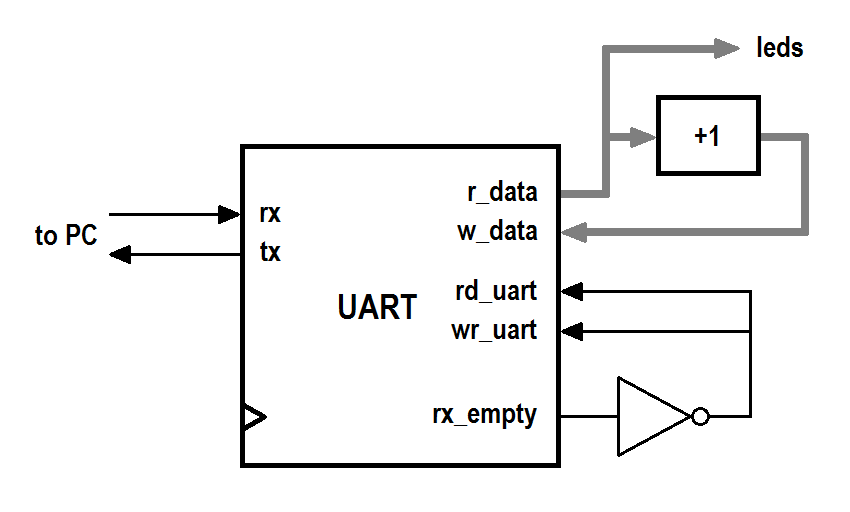
\includegraphics[width=0.6\textwidth]{test_fig}
\caption{Некий рисунок}
\label{test_fig_label}
\end{figure}
